\acao{Ação 3.2.2.7 – Supervisão e gerenciamento das obras}

\phantomsection
\addcontentsline{toc}{subsection}{1. Contextualização}
\subsection*{1. Contextualização}

A ação contrata empresa de supervisão e gerenciamento para o acompanhamento independente das obras de abastecimento de água e de esgotamento sanitário da atividade, em apoio à fiscalização do IAT, com registro do andamento, da qualidade e da conformidade ambiental e social das obras (IAT, 2026a).

As obras da atividade são numerosas e dispersas no território estadual: 83 sistemas coletivos de abastecimento de água e 6.367 instalações domiciliares de esgotamento sanitário. A equipe de fiscalização do IAT não tem capacidade para acompanhar simultaneamente todas as frentes, e a ausência de acompanhamento contínuo eleva os riscos de atraso, de não conformidade e de pagamento sem comprovação suficiente.

A supervisão confere qualidade e rastreabilidade às obras: os relatórios e as medições verificadas pela supervisora subsidiam os critérios de aceite, os pagamentos e a emissão do Termo de Recebimento Definitivo nas ações de abastecimento de água e de esgotamento sanitário.

\textbf{Inclui:} o plano de supervisão; o acompanhamento de campo; o controle de qualidade dos materiais e dos serviços; a verificação das medições; o controle de prazos e custos; a verificação da conformidade ambiental, social e de saúde e segurança do trabalho; os relatórios mensais; e o apoio ao recebimento das obras.

\textbf{Não inclui:} a fiscalização dos contratos, que permanece atribuição do IAT, nem os projetos e as obras.

\textbf{Valor previsto:} R\$~10,79 milhões (empréstimo BIRD: R\$~10,79 milhões; contrapartida: R\$~0,00 milhões), conforme a planilha PSH\_CUSTO\_Consolidada.

\phantomsection
\addcontentsline{toc}{subsection}{2. Área de atuação}
\subsection*{2. Área de atuação}

A supervisão abrange todas as frentes de obra da atividade: as 83 comunidades atendidas com abastecimento de água e esgotamento sanitário (Figura~\ref{mapa}) e as propriedades dos nove mananciais selecionados (Tabela~\ref{mananciais}).

\phantomsection
\addcontentsline{toc}{subsection}{3. Arranjo institucional e partes interessadas}
\subsection*{3. Arranjo institucional e partes interessadas}

O IAT, por meio da DISAR, contrata a supervisora, designa a fiscalização de cada contrato de obra e aprova os relatórios. A supervisora acompanha as obras e reporta ao IAT, e os executores das obras corrigem as não conformidades apontadas. A UGP recebe as informações de progresso físico e de conformidade ambiental e social, e o Banco Mundial manifesta-se sobre o Termo de Referência e a seleção, quando houver revisão prévia.

\begin{itemize}
  \item \textbf{Intervenientes:} empresa supervisora; empresas executoras das obras; prefeituras, informadas do andamento;
  \item \textbf{Público envolvido:} moradores das comunidades e proprietários das áreas com obras.
\end{itemize}

Os beneficiários diretos são o IAT, que amplia a capacidade de acompanhamento das obras, e as comunidades, que recebem obras de melhor qualidade. Os beneficiários indiretos são os usuários dos sistemas e o Programa, com a redução dos riscos de execução.

\phantomsection
\addcontentsline{toc}{subsection}{4. Processo de execução operacional}
\subsection*{4. Processo de execução operacional}

A ação compreende cinco etapas, da contratação ao relatório final (Figura~\ref{raias-3227}). Durante as obras, a supervisão opera em ciclo mensal (Figura~\ref{ciclo-supervisao}): visitas de campo e controle de qualidade, correção das não conformidades pelo executor, verificação das medições, relatório mensal aprovado pelo IAT e consolidação do progresso pela UGP.

\begin{figure}[H]
  \centering
  \caption{Fluxograma da supervisão e gerenciamento das obras: entradas, etapas por responsável e saídas}\label{raias-3227}
  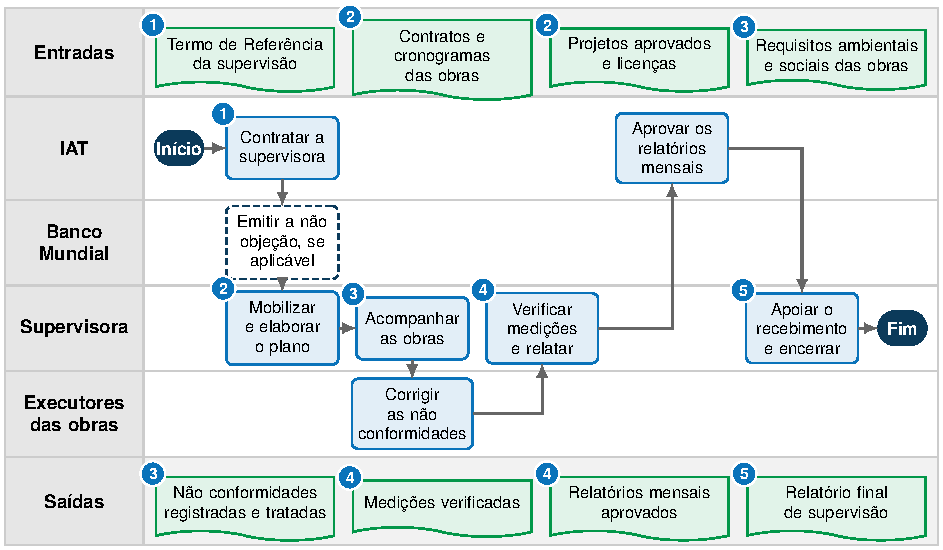
\includegraphics[width=15.96cm]{figuras/g-raias-3227.pdf}
  \fonteMOP{Fonte: IAT (2026).}
  % Texto alternativo: Fluxograma em raias da supervisão e gerenciamento das obras, com uma raia por instituição, as etapas numeradas na raia do executor, as entradas no topo e as saídas na base.
\end{figure}

\begin{figure}[H]
  \centering
  \caption{Ciclo mensal de supervisão das obras}\label{ciclo-supervisao}
  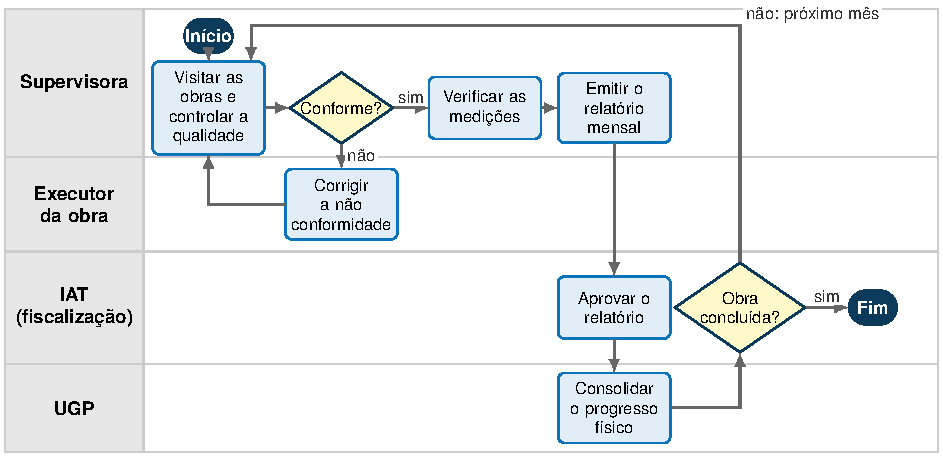
\includegraphics[width=15.96cm]{figuras/f-ciclo-supervisao.pdf}
  \fonteMOP{Fonte: IAT (2026).}
  % Texto alternativo: Fluxograma em raias do ciclo mensal de supervisão, com a correção das não conformidades, a aprovação do relatório pelo IAT, a consolidação pela UGP e a repetição mensal até a conclusão das obras.
\end{figure}

\phantomsection
\subsubsection*{4.1 Etapa 1: Contratação da supervisora}

\textbf{Atividades:} elaboração do Termo de Referência, com escopo, equipe e produtos; seleção da consultoria pelo método definido no Plano de Aquisições; assinatura do contrato e emissão da ordem de serviço.

\textbf{Entradas:} cronogramas previstos das obras; Termo de Referência.

\textbf{Responsáveis:} IAT (executa e aprova); UGP e Banco Mundial (consultados).

\textbf{Produto:} contrato assinado.

\phantomsection
\subsubsection*{4.2 Etapa 2: Mobilização e plano de supervisão}

\textbf{Atividades:} mobilização da equipe; elaboração do plano de supervisão, com procedimentos de medição, de controle de qualidade e de registro das não conformidades; implantação do sistema de registro e de relatórios.

\textbf{Entradas:} contrato; projetos aprovados; contratos das obras.

\textbf{Responsáveis:} supervisora (executa); IAT (aprova).

\textbf{Produto:} plano de supervisão aprovado.

\phantomsection
\subsubsection*{4.3 Etapa 3: Acompanhamento das obras}

\textbf{Atividades:} visitas de campo; controle de qualidade dos materiais e dos serviços; verificação dos requisitos ambientais, sociais e de saúde e segurança do trabalho; registro das não conformidades e acompanhamento da correção.

\textbf{Entradas:} plano de supervisão; obras em execução.

\textbf{Responsáveis:} supervisora (executa); executores das obras (corrigem); IAT (aprova).

\textbf{Produto:} registros de campo e de não conformidades.

\phantomsection
\subsubsection*{4.4 Etapa 4: Medições e relatórios}

\textbf{Atividades:} verificação das medições dos executores; controle de prazos e custos; relatórios mensais ao IAT, com as informações de progresso destinadas à UGP.

\textbf{Entradas:} registros de campo; medições dos executores.

\textbf{Responsáveis:} supervisora (executa); IAT (aprova); UGP (informada).

\textbf{Produto:} relatórios mensais aprovados.

\phantomsection
\subsubsection*{4.5 Etapa 5: Recebimento das obras e encerramento}

\textbf{Atividades:} apoio ao recebimento provisório e definitivo das obras; conferência dos projetos \textit{as built}; relatório final de supervisão.

\textbf{Entradas:} obras concluídas; relatórios mensais.

\textbf{Responsáveis:} supervisora (executa); IAT (aprova).

\textbf{Produto:} relatório final de supervisão.

\phantomsection
\subsubsection*{4.6 Modalidade de execução}

O item de custo é a supervisão e o gerenciamento de obras: 36 profissionais-mês a R\$~299.722,20, no total de R\$~10,79 milhões, com recursos do empréstimo do BIRD. A execução ocorre mediante licitação de serviços de consultoria, conforme o Caderno AQ.

\pendencia{A supervisão está prevista de 2029 a 2032, e as obras de abastecimento estendem-se de 2028 a 2033. Avaliar a supervisão das obras de 2028 e de 2033 e confirmar se o escopo inclui as instalações de esgotamento sanitário.}

\phantomsection
\addcontentsline{toc}{subsection}{5. Matriz de responsabilidades}
\subsection*{5. Matriz de responsabilidades}

O Quadro~\ref{raci-3227} apresenta o papel de cada parte em cada etapa.

\begin{quadro}[H]
  \caption{Matriz de responsabilidades da supervisão e gerenciamento das obras}\label{raci-3227}
  \footnotesize\renewcommand{\arraystretch}{1.25}\setlength{\tabcolsep}{3pt}
  \begin{tabular}{>{\raggedright\arraybackslash}p{\dimexpr 0.2536\linewidth-2\tabcolsep\relax}>{\centering\arraybackslash}p{\dimexpr 0.0882\linewidth-2\tabcolsep\relax}>{\centering\arraybackslash}p{\dimexpr 0.0882\linewidth-2\tabcolsep\relax}>{\centering\arraybackslash}p{\dimexpr 0.0882\linewidth-2\tabcolsep\relax}>{\centering\arraybackslash}p{\dimexpr 0.0882\linewidth-2\tabcolsep\relax}>{\centering\arraybackslash}p{\dimexpr 0.0882\linewidth-2\tabcolsep\relax}>{\centering\arraybackslash}p{\dimexpr 0.3055\linewidth-2\tabcolsep\relax}}
    \rowcolor{azulEscuro}\textcolor{white}{\textbf{Parte}} & \textcolor{white}{\textbf{E1}} & \textcolor{white}{\textbf{E2}} & \textcolor{white}{\textbf{E3}} & \textcolor{white}{\textbf{E4}} & \textcolor{white}{\textbf{E5}} & \textcolor{white}{\textbf{Produto final}} \\
    IAT & \raci{R} \raci{A} & \raci{A} & \raci{A} & \raci{A} & \raci{A} & \raci{A} \\ \arrayrulecolor{cinza20}\hline
    \rowcolor{cinza5}Supervisora & – & \raci{R} & \raci{R} & \raci{R} & \raci{R} & \raci{R} \\ \arrayrulecolor{cinza20}\hline
    Executores das obras & – & \raci{C} & \raci{R} & \raci{C} & \raci{C} & \raci{I} \\ \arrayrulecolor{cinza20}\hline
    \rowcolor{cinza5}Prefeituras & – & \raci{I} & \raci{I} & – & \raci{I} & \raci{I} \\ \arrayrulecolor{cinza20}\hline
    UGP & \raci{C} & \raci{I} & \raci{I} & \raci{I} & \raci{I} & \raci{I} \\ \arrayrulecolor{cinza20}\hline
    \rowcolor{cinza5}Banco Mundial & \raci{C} & – & – & – & – & – \\ \noalign{\global\arrayrulewidth=1pt}\arrayrulecolor{azulEscuro}\hline\noalign{\global\arrayrulewidth=0.4pt}
  \end{tabular}
  \fonteMOP{Fonte: IAT (2026).}
  \notaMOP{Nota: E1 a E5 correspondem às Etapas 1 a 5 do item 4. \raci{R} executa (pode haver mais de um); \raci{A} aprova ou valida o produto (um por etapa); \raci{C} é consultado previamente; \raci{I} é informado posteriormente. Produto final: obras supervisionadas, com relatórios aprovados.}
\end{quadro}

\phantomsection
\addcontentsline{toc}{subsection}{6. Metas, indicadores e comprovação}
\subsection*{6. Metas, indicadores e comprovação}

A meta física é expressa em profissionais-mês, de 2029 a 2032 (Quadro~\ref{metas-3227}).

\begin{quadro}[H]
  \caption{Metas anuais da supervisão e gerenciamento das obras}\label{metas-3227}
  \footnotesize\renewcommand{\arraystretch}{1.25}\setlength{\tabcolsep}{3pt}
  \begin{tabular}{>{\raggedright\arraybackslash}p{\dimexpr 0.2095\linewidth-2\tabcolsep\relax}>{\raggedright\arraybackslash}p{\dimexpr 0.1268\linewidth-2\tabcolsep\relax}>{\raggedleft\arraybackslash}p{\dimexpr 0.0794\linewidth-2\tabcolsep\relax}>{\raggedleft\arraybackslash}p{\dimexpr 0.0794\linewidth-2\tabcolsep\relax}>{\raggedleft\arraybackslash}p{\dimexpr 0.0794\linewidth-2\tabcolsep\relax}>{\raggedleft\arraybackslash}p{\dimexpr 0.0794\linewidth-2\tabcolsep\relax}>{\raggedleft\arraybackslash}p{\dimexpr 0.0794\linewidth-2\tabcolsep\relax}>{\raggedleft\arraybackslash}p{\dimexpr 0.0794\linewidth-2\tabcolsep\relax}>{\raggedleft\arraybackslash}p{\dimexpr 0.0794\linewidth-2\tabcolsep\relax}>{\raggedleft\arraybackslash}p{\dimexpr 0.1081\linewidth-2\tabcolsep\relax}}
    \rowcolor{azulEscuro}\textcolor{white}{\textbf{Produto}} & \textcolor{white}{\textbf{Unidade}} & \centering\arraybackslash \textcolor{white}{\textbf{Ano 1}} & \centering\arraybackslash \textcolor{white}{\textbf{Ano 2}} & \centering\arraybackslash \textcolor{white}{\textbf{Ano 3}} & \centering\arraybackslash \textcolor{white}{\textbf{Ano 4}} & \centering\arraybackslash \textcolor{white}{\textbf{Ano 5}} & \centering\arraybackslash \textcolor{white}{\textbf{Ano 6}} & \centering\arraybackslash \textcolor{white}{\textbf{Ano 7}} & \centering\arraybackslash \textcolor{white}{\textbf{Total}} \\
    Supervisão e gerenciamento de obras & prof.-mês & – & – & 6 & 12 & 12 & 6 & – & 36 \\ \noalign{\global\arrayrulewidth=1pt}\arrayrulecolor{azulEscuro}\hline\noalign{\global\arrayrulewidth=0.4pt}
  \end{tabular}
  \fonteMOP{Fonte: Planilha PSH\_CUSTO\_Consolidada, versão v2408 (PARANÁ, 2026).}
  \notaMOP{Nota: Ano 1 = 2027 e Ano 7 = 2033. Prof.-mês = profissionais-mês.}
\end{quadro}

Os indicadores constam do Quadro~\ref{ind-3227}, e os critérios de aceite, do Quadro~\ref{aceite-3227}.

\begin{quadro}[H]
  \caption{Indicadores da supervisão e gerenciamento das obras}\label{ind-3227}
  \footnotesize\renewcommand{\arraystretch}{1.25}\setlength{\tabcolsep}{3pt}
  \begin{tabular}{>{\raggedright\arraybackslash}p{\dimexpr 0.3165\linewidth-2\tabcolsep\relax}>{\raggedright\arraybackslash}p{\dimexpr 0.1378\linewidth-2\tabcolsep\relax}>{\raggedleft\arraybackslash}p{\dimexpr 0.1102\linewidth-2\tabcolsep\relax}>{\raggedleft\arraybackslash}p{\dimexpr 0.1599\linewidth-2\tabcolsep\relax}>{\raggedright\arraybackslash}p{\dimexpr 0.2756\linewidth-2\tabcolsep\relax}}
    \rowcolor{azulEscuro}\textcolor{white}{\textbf{Indicador}} & \textcolor{white}{\textbf{Unidade}} & \centering\arraybackslash \textcolor{white}{\textbf{Linha de base (2025)}} & \centering\arraybackslash \textcolor{white}{\textbf{Meta}} & \textcolor{white}{\textbf{Frequência e fonte dos dados}} \\
    Relatórios de supervisão aprovados & relatórios & 0 & 1 por mês de supervisão & Mensal; IAT \\ \arrayrulecolor{cinza20}\hline
    \rowcolor{cinza5}Sistemas de abastecimento supervisionados com Termo de Recebimento Definitivo & sistemas & 0 & 83 & Semestral; IAT \\ \arrayrulecolor{cinza20}\hline
    Não conformidades corrigidas no prazo & \% das registradas & – & 100 & Mensal; relatórios de supervisão \\ \noalign{\global\arrayrulewidth=1pt}\arrayrulecolor{azulEscuro}\hline\noalign{\global\arrayrulewidth=0.4pt}
  \end{tabular}
  \fonteMOP{Fonte: IAT (2026).}
\end{quadro}

\pendencia{Definir no Termo de Referência o número de relatórios e a distribuição dos 36 profissionais-mês entre as frentes de obra.}

\begin{quadro}[H]
  \caption{Critérios de aceite e evidências da supervisão e gerenciamento das obras}\label{aceite-3227}
  \footnotesize\renewcommand{\arraystretch}{1.25}\setlength{\tabcolsep}{5pt}
  \begin{tabular}{>{\raggedright\arraybackslash}p{\dimexpr 0.2150\linewidth-2\tabcolsep\relax}>{\raggedright\arraybackslash}p{\dimexpr 0.3386\linewidth-2\tabcolsep\relax}>{\raggedright\arraybackslash}p{\dimexpr 0.2921\linewidth-2\tabcolsep\relax}>{\raggedright\arraybackslash}p{\dimexpr 0.1543\linewidth-2\tabcolsep\relax}}
    \rowcolor{azulEscuro}\textcolor{white}{\textbf{Produto}} & \textcolor{white}{\textbf{Critério de aceite}} & \textcolor{white}{\textbf{Evidência de comprovação}} & \textcolor{white}{\textbf{Responsável pela validação}} \\
    Plano de supervisão & Procedimentos de medição, qualidade e registro definidos & Plano aprovado & IAT \\ \arrayrulecolor{cinza20}\hline
    \rowcolor{cinza5}Relatório mensal & Andamento, medições, não conformidades e conformidade ambiental e social de cada frente & Relatório aprovado & IAT \\ \arrayrulecolor{cinza20}\hline
    Medições verificadas & Quantidades conferidas em campo & Boletins de medição atestados & IAT \\ \arrayrulecolor{cinza20}\hline
    \rowcolor{cinza5}Relatório final & Consolida a supervisão e o recebimento das obras & Relatório final aprovado & IAT \\ \noalign{\global\arrayrulewidth=1pt}\arrayrulecolor{azulEscuro}\hline\noalign{\global\arrayrulewidth=0.4pt}
  \end{tabular}
  \fonteMOP{Fonte: IAT (2026).}
\end{quadro}

\phantomsection
\addcontentsline{toc}{subsection}{7. Gestão de riscos e impactos ambientais e sociais}
\subsection*{7. Gestão de riscos e impactos ambientais e sociais}

A supervisora constitui instrumento de cumprimento das NAS nas obras, mediante verificação em campo dos requisitos ambientais, sociais e de saúde e segurança aplicáveis às ações de abastecimento de água e de esgotamento sanitário (Quadro~\ref{nas-3227}). As demais NAS são tratadas nas respectivas ações.

\begin{quadro}[H]
  \caption{Aplicação das Normas Ambientais e Sociais à supervisão e gerenciamento das obras}\label{nas-3227}
  \footnotesize\renewcommand{\arraystretch}{1.25}\setlength{\tabcolsep}{5pt}
  \begin{tabular}{>{\raggedright\arraybackslash}p{\dimexpr 0.1874\linewidth-2\tabcolsep\relax}>{\raggedright\arraybackslash}p{\dimexpr 0.3716\linewidth-2\tabcolsep\relax}>{\raggedright\arraybackslash}p{\dimexpr 0.4410\linewidth-2\tabcolsep\relax}}
    \rowcolor{azulEscuro}\textcolor{white}{\textbf{NAS}} & \textcolor{white}{\textbf{Aplicação à ação}} & \textcolor{white}{\textbf{Medidas e instrumentos}} \\
    NAS 1 – Avaliação e gestão de riscos & Acompanhamento dos planos ambientais e sociais das obras & Verificação e registro em cada relatório mensal (MGAS) \\ \arrayrulecolor{cinza20}\hline
    \rowcolor{cinza5}NAS 2 – Condições de trabalho & Trabalhadores das obras e da própria supervisora & Verificação de EPI, treinamentos e registros de incidentes (Procedimentos de Gestão de Mão de Obra) \\ \arrayrulecolor{cinza20}\hline
    NAS 4 – Saúde e segurança da comunidade & Sinalização e isolamento das obras nas comunidades & Inspeção de campo e exigência de correção imediata \\ \arrayrulecolor{cinza20}\hline
    \rowcolor{cinza5}NAS 10 – Engajamento das partes interessadas & Queixas relacionadas às obras & Registro e encaminhamento ao Mecanismo de Queixas e Reclamações (MQR) \\ \noalign{\global\arrayrulewidth=1pt}\arrayrulecolor{azulEscuro}\hline\noalign{\global\arrayrulewidth=0.4pt}
  \end{tabular}
  \fonteMOP{Fonte: IAT (2026), com base nos instrumentos do Caderno AS.}
\end{quadro}

\phantomsection
\addcontentsline{toc}{subsection}{8. Cronograma}
\subsection*{8. Cronograma}

A contratação ocorre em 2028, a mobilização em 2029 e a supervisão de 2029 a 2032, com 6 profissionais-mês em 2029, 12 em 2030 e em 2031 e 6 em 2032 (Figura~\ref{crono-3227}).

\begin{figure}[H]
  \centering
  \caption{Cronograma das etapas e das entregas da supervisão e gerenciamento das obras}\label{crono-3227}
  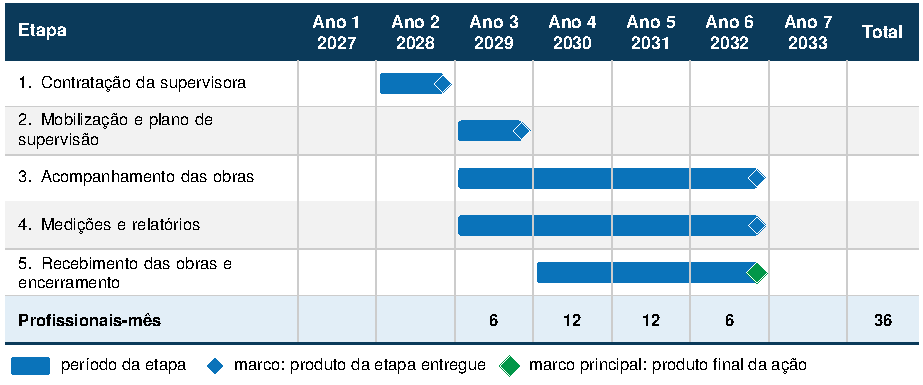
\includegraphics[width=15.64cm]{figuras/g-crono-3227.pdf}
  \fonteMOP{Fonte: IAT (2026), com quantidades da planilha PSH\_CUSTO\_Consolidada (PARANÁ, 2026).}
  % Texto alternativo: Cronograma anual de 2027 a 2033 com as etapas e as quantidades a entregar da supervisão e gerenciamento das obras.
\end{figure}

\phantomsection
\addcontentsline{toc}{subsection}{9. Interfaces e dependências}
\subsection*{9. Interfaces e dependências}

A ação depende dos contratos, dos projetos e dos cronogramas das obras de abastecimento de água e de esgotamento sanitário. Fornece ao IAT os relatórios que fundamentam as medições, os pagamentos e o recebimento das obras, aos executores as não conformidades a corrigir e à UGP as informações de progresso físico e de conformidade (Figura~\ref{interf-3227}).

\begin{figure}[H]
  \centering
  \caption{Interfaces e dependências da supervisão e gerenciamento das obras}\label{interf-3227}
  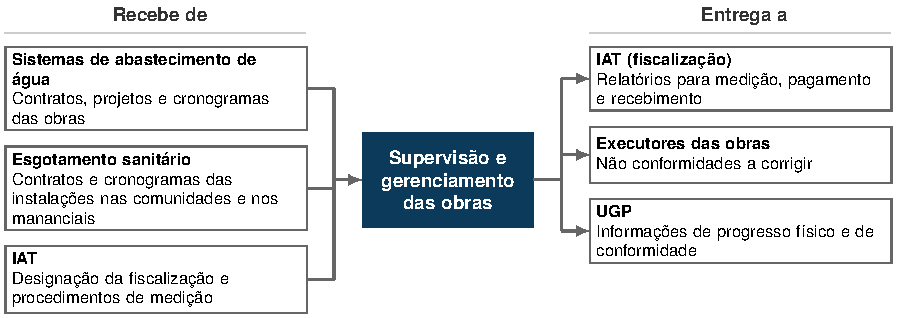
\includegraphics[width=15.30cm]{figuras/g-interf-3227.pdf}
  \fonteMOP{Fonte: IAT (2026).}
  % Texto alternativo: Diagrama das interfaces da supervisão e gerenciamento das obras: insumos recebidos de outras partes do Programa e produtos entregues a elas.
\end{figure}

\phantomsection
\addcontentsline{toc}{subsection}{10. Documentos complementares}
\subsection*{10. Documentos complementares}

\begin{itemize}
  \item Termo de Referência da supervisão e do gerenciamento das obras (a elaborar);
  \item Regulamento de Aquisições do Banco Mundial para mutuários de Financiamento de Projetos de Investimento e Caderno AQ;
  \item Caderno AS;
  \item Normas técnicas aplicáveis às obras (ABNT) e projetos aprovados de cada sistema.
\end{itemize}
